% !TeX root = document-en.tex

\chapter{Related Works}
\label{related}

\makeendnotes  %make notes at the last of this chapter // if you do not  want use endnotes style, please comment out this.

\section{Shifting to Creative Society}
\subsection{A WHOLE NEW MIND}


\section{Design Thinking Workshop}
\subsection{IDEO}
We also ate riceand bread.

\subsection{d-school}
Also Pink  said something about creativity.


\subsection{SDM}
Recently SDM is also conducting design thinking workshop in the Collaboration Complex\footnote{Graduate School of System Design and Management, Keio University \\\url{http://www.sdm.keio.ac.jp/}}. But {\it iias Tsukuba} (Figure \ref{iias})\footnote{{\it iias Tsukuba} is one of largest shopping center located in Tsukuba city. \url{http://tsukuba.iias.jp}} has not conducted design thinking workshop yet. 


%inputting jpg
\begin{figure}[htbp]
\centering
  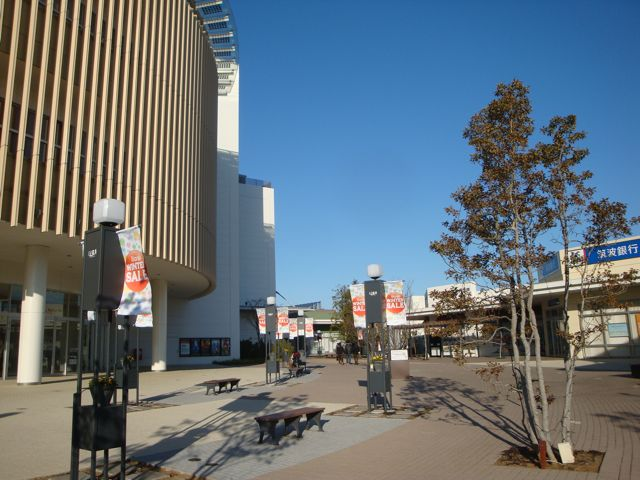
\includegraphics[width=85mm, bb=0 0 640 480]{figures/iias.jpg}
 \caption{Shopping center {\itshape iiasTsukuba}}
  \label{iias}
\end{figure}


%inputting tables
\begin{table}[ht]
\caption{state of your mind}
\label{cluster_category}
\centering
\small
\begin{tabu} to \linewidth {|c|c|c|c|}
\hline
% setting the size of the grid (only necessary if you want absolute column sizes)
\makebox[8em][c]{when} &
\makebox[8em][c]{where} &
\makebox[8em][c]{who} &
\makebox[8em][c]{what}\\
\hline
Bad & Good & Very Good & Good Good\\
\hline
\end{tabu}
\end{table}


%%%%%Notes%%%%%
% if you do not  want use endnotes style, please comment out the below.
\section*{Notes}
\addcontentsline{toc}{section}{Notes}
\begin{footnotesize}
\theendnotes
\end{footnotesize}
